\documentclass[
  bibliography=totoc,     % Literatur im Inhaltsverzeichnis
  captions=tableheading,  % Tabellenüberschriften
  titlepage=firstiscover, % Titelseite ist Deckblatt
]{scrartcl}

% Paket float verbessern
\usepackage{scrhack}

% Warnung, falls nochmal kompiliert werden muss
\usepackage[aux]{rerunfilecheck}

% unverzichtbare Mathe-Befehle
\usepackage{amsmath}
% viele Mathe-Symbole
\usepackage{amssymb}
% Erweiterungen für amsmath
\usepackage{mathtools}

% Fonteinstellungen
\usepackage{fontspec}
% Latin Modern Fonts werden automatisch geladen
% Alternativ zum Beispiel:
%\setromanfont{Libertinus Serif}
%\setsansfont{Libertinus Sans}
%\setmonofont{Libertinus Mono}

% Wenn man andere Schriftarten gesetzt hat,
% sollte man das Seiten-Layout neu berechnen lassen
\recalctypearea{}

% deutsche Spracheinstellungen
\usepackage[ngerman]{babel}


\usepackage[
  math-style=ISO,    % ┐
  bold-style=ISO,    % │
  sans-style=italic, % │ ISO-Standard folgen
  nabla=upright,     % │
  partial=upright,   % │
  mathrm=sym,        % ┘
  warnings-off={           % ┐
    mathtools-colon,       % │ unnötige Warnungen ausschalten
    mathtools-overbracket, % │
  },                       % ┘
]{unicode-math}

% traditionelle Fonts für Mathematik
\setmathfont{Latin Modern Math}
% Alternativ zum Beispiel:
%\setmathfont{Libertinus Math}

\setmathfont{XITS Math}[range={scr, bfscr}]
\setmathfont{XITS Math}[range={cal, bfcal}, StylisticSet=1]

% Zahlen und Einheiten
\usepackage[
  locale=DE,                   % deutsche Einstellungen
  separate-uncertainty=true,   % immer Unsicherheit mit \pm
  per-mode=symbol-or-fraction, % / in inline math, fraction in display math
]{siunitx}

% chemische Formeln
\usepackage[
  version=4,
  math-greek=default, % ┐ mit unicode-math zusammenarbeiten
  text-greek=default, % ┘
]{mhchem}

% richtige Anführungszeichen
\usepackage[autostyle]{csquotes}

% schöne Brüche im Text
\usepackage{xfrac}

% Standardplatzierung für Floats einstellen
\usepackage{float}
\floatplacement{figure}{htbp}
\floatplacement{table}{htbp}

% Floats innerhalb einer Section halten
\usepackage[
  section, % Floats innerhalb der Section halten
  below,   % unterhalb der Section aber auf der selben Seite ist ok
]{placeins}

% Seite drehen für breite Tabellen: landscape Umgebung
\usepackage{pdflscape}

% Captions schöner machen.
\usepackage[
  labelfont=bf,        % Tabelle x: Abbildung y: ist jetzt fett
  font=small,          % Schrift etwas kleiner als Dokument
  width=0.9\textwidth, % maximale Breite einer Caption schmaler
]{caption}
% subfigure, subtable, subref
\usepackage{subcaption}

% Grafiken können eingebunden werden
\usepackage{graphicx}

% schöne Tabellen
\usepackage{tabularray}
\UseTblrLibrary{booktabs, siunitx}

% Verbesserungen am Schriftbild
\usepackage{microtype}

% Literaturverzeichnis
\usepackage[
  backend=biber,
]{biblatex}
% Quellendatenbank
\addbibresource{lit.bib}
\addbibresource{programme.bib}

% Hyperlinks im Dokument
\usepackage[
  german,
  unicode,        % Unicode in PDF-Attributen erlauben
  pdfusetitle,    % Titel, Autoren und Datum als PDF-Attribute
  pdfcreator={},  % ┐ PDF-Attribute säubern
  pdfproducer={}, % ┘
]{hyperref}
% erweiterte Bookmarks im PDF
\usepackage{bookmark}

% Trennung von Wörtern mit Strichen
\usepackage[shortcuts]{extdash}

\author{%
  Vincent Wirsdörfer\\%
  \href{mailto:vincent.wirsdoerfer@udo.edu}{authorA@udo.edu}%
  \and%
  Joris Daus\\%
  \href{mailto:joris.daus@udo.edu}{authorB@udo.edu}%
}
\publishers{TU Dortmund – Fakultät Physik}


\begin{document}
\section{Versuchsaufbau}
Im Folgenden wird der Versuchsaufbau aus \autoref{fig:Aufbau} erklärt, indem zunächst der Strahlengang erläutert wird.\\

\begin{figure}[H]
    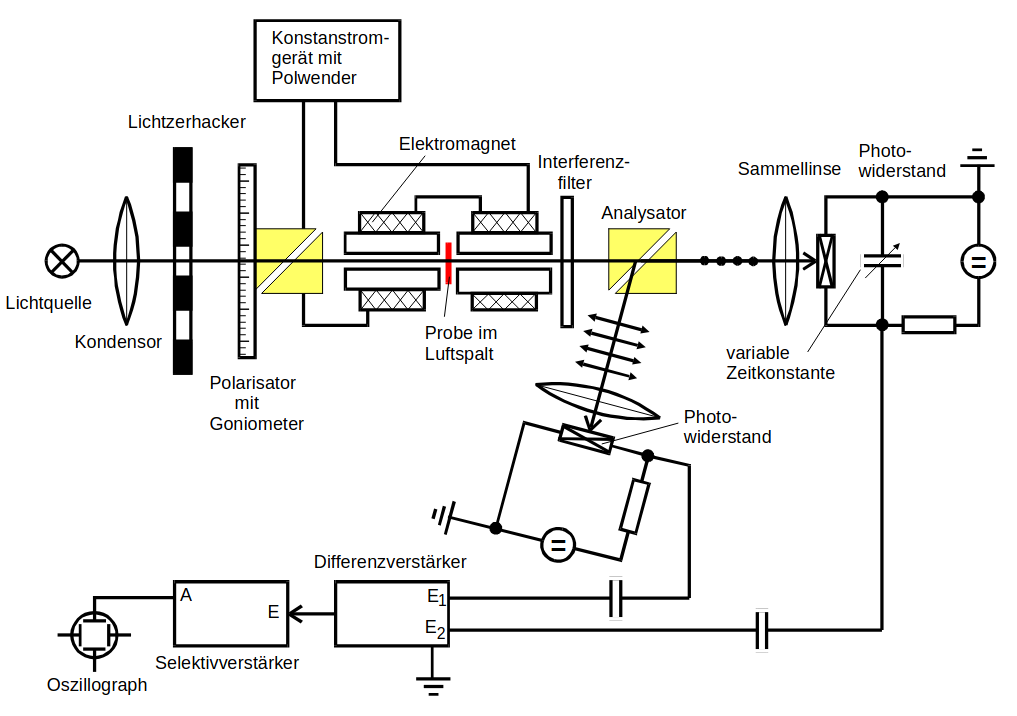
\includegraphics[width=0.9\textwidth]{Aufbau.png}
    \caption{Schematischer Aufbau des Versuches \cite{Versuchsanleitung_v46}.}
    \label{fig:Aufbau}
\end{figure}

\noindent Die Lichtquelle stellt eine Halogenlampe dar, welche mit \qty{7}{\volt} und \qty{3.2}{\ampere} betrieben wird.
Das Licht der Lampe wird durch eine Linse parallelisiert, sodass die Intensität über die Länge des Versuchsaufbaus erhalten bleibt. 
Hinter der Linse steht ein Chopper, welcher das Lichtsignal zerhackt. Im Anschluss steht das erste Glan-Thompson-Prisma, welches mit 
einem Goniometer verbunden ist und das durchgehende Licht linear polarisiert. Die Drehachse liegt entlang der Ausbreitungsrichtung. 
Der linear polarisierte Lichtstrahl geht längs des Magnetes durch eine Bohrung. Die Magnetfeldlinien liegen somit parallel zum 
Lichtstrahl. Wie in der \autoref{fig:Schlitz} zu sehen ist, ist in der Mitte des Magnets ein Schlitz, in welchem die GaAs Probe eingelegt 
werden kann.

\begin{figure}[H]
    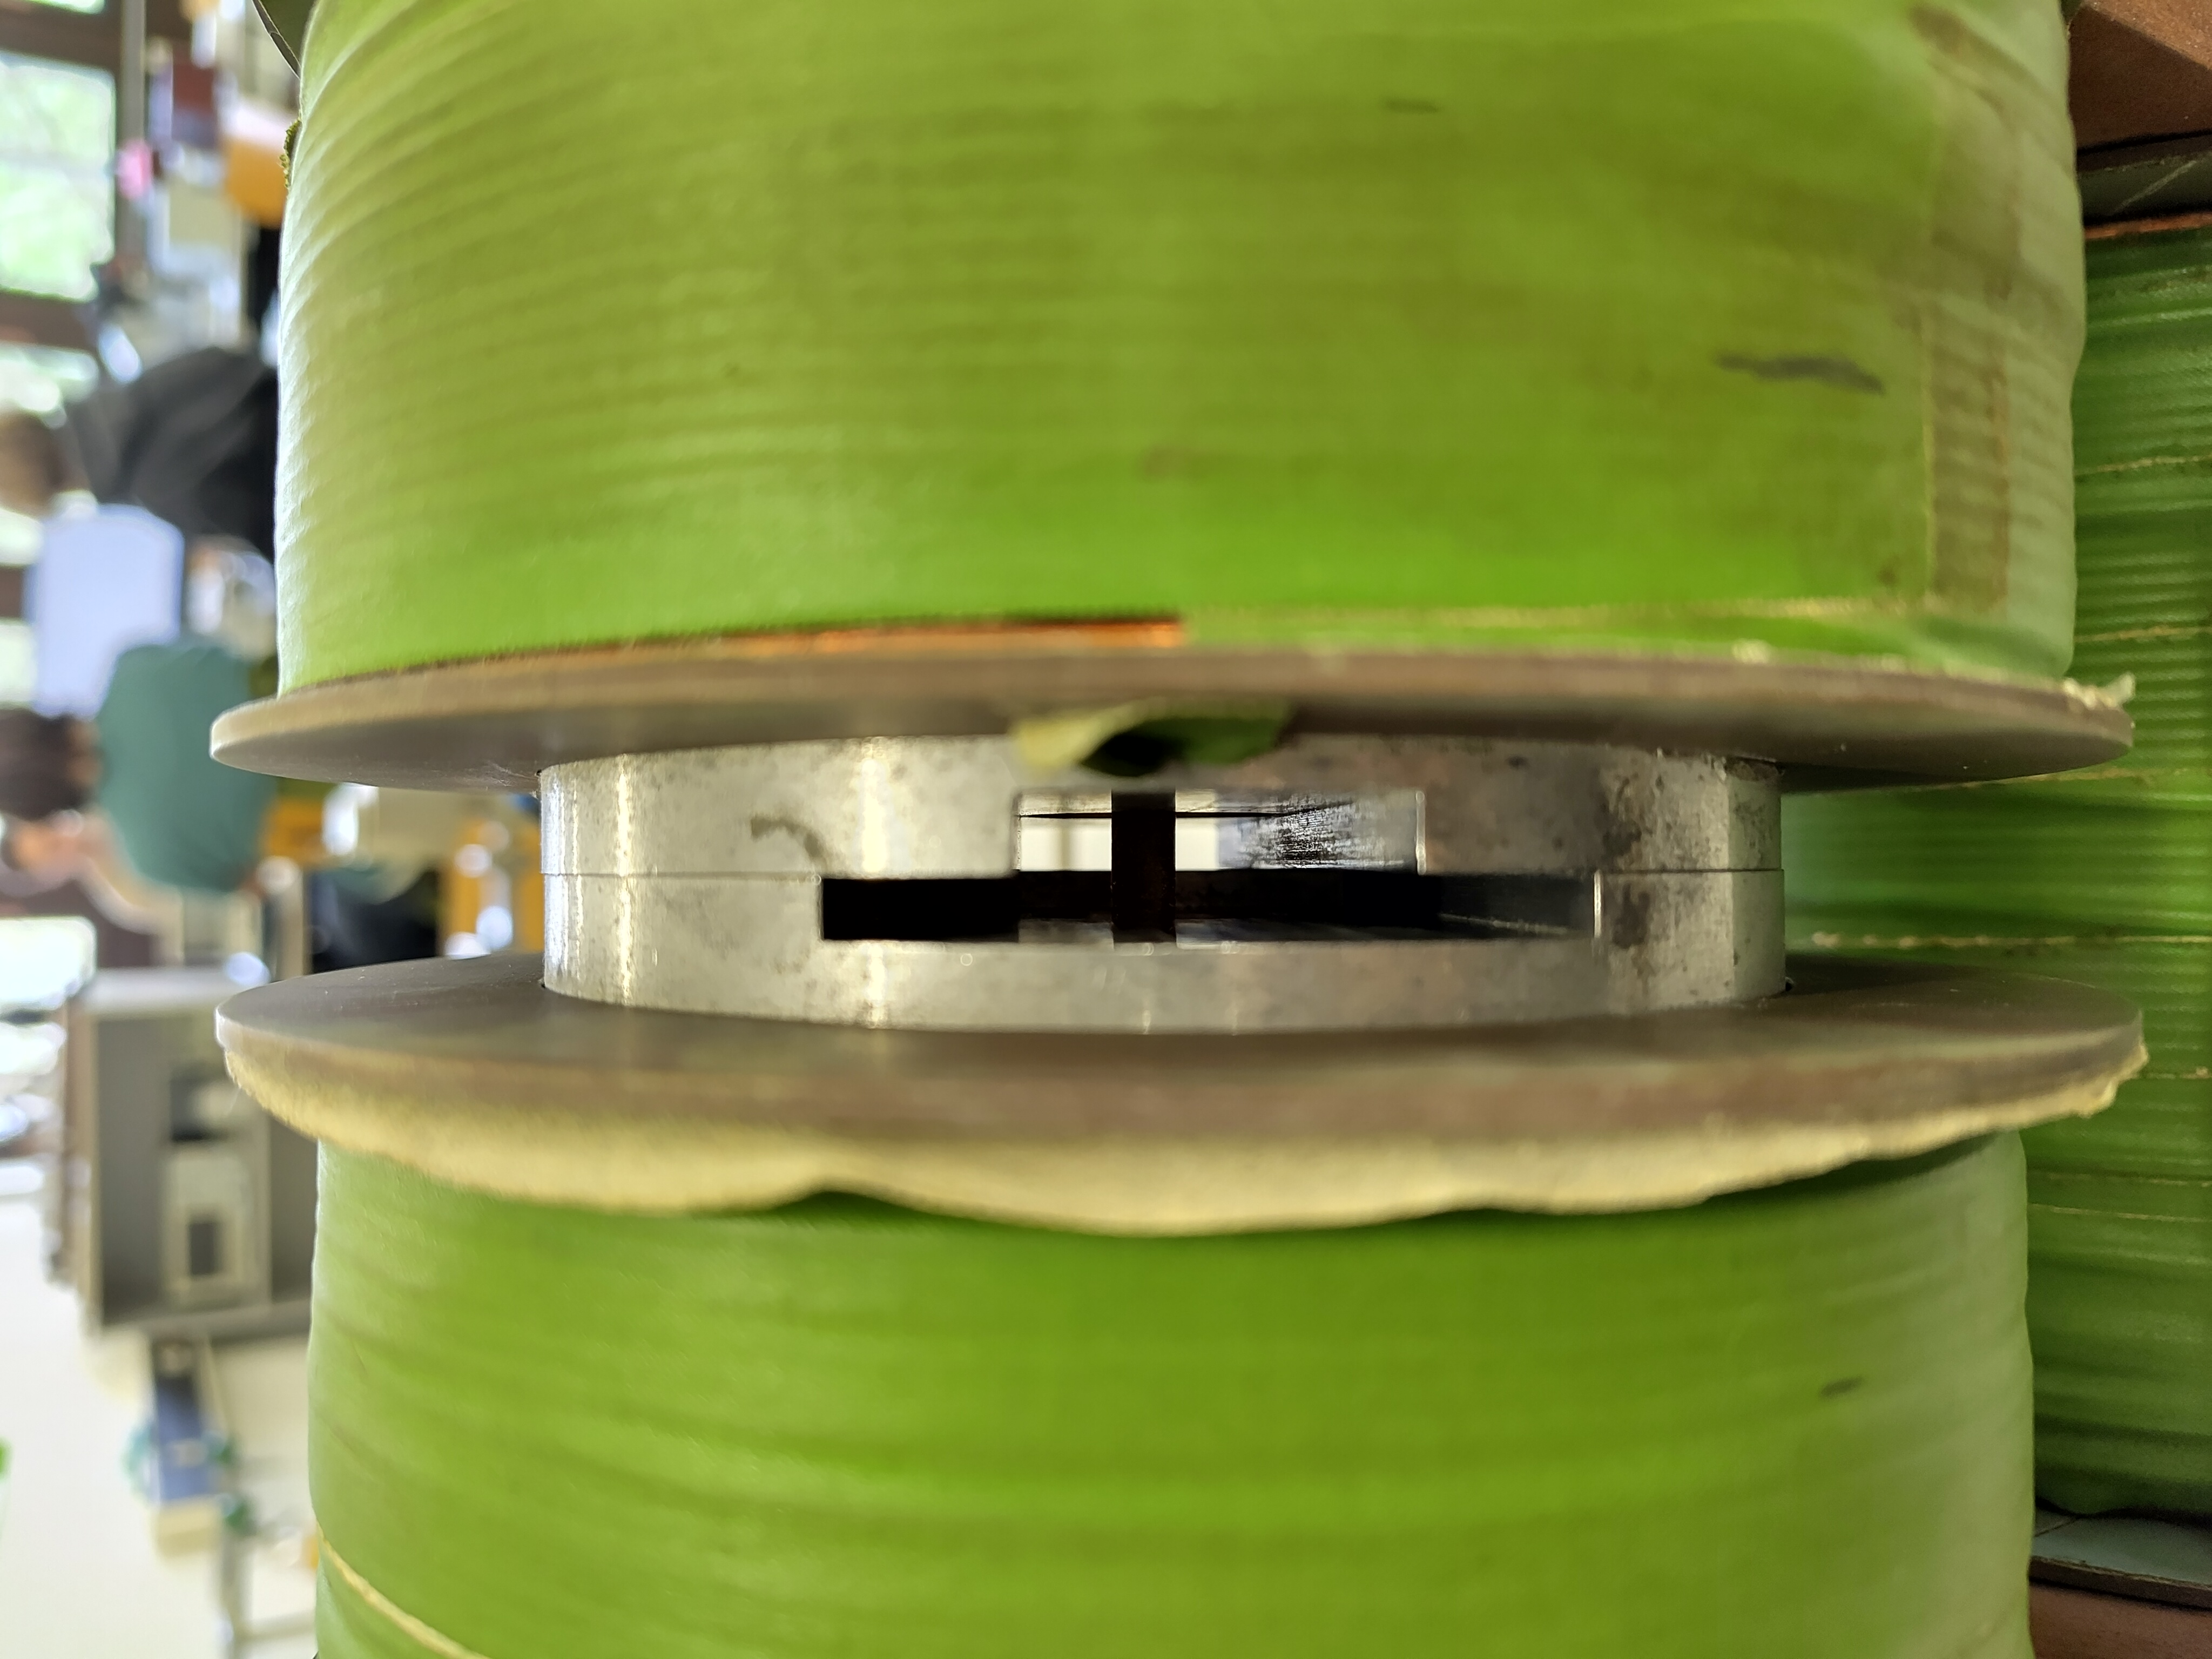
\includegraphics[width=0.5\textwidth]{Schlitz.jpg}
    \caption{Schlitz für die Probe im Magneten.}
    \label{fig:Schlitz}
\end{figure}

\noindent Hinter dem Magneten steht nun ein Interferenzfilter, welcher alle Wellenlängen bis auf eine herausfiltert. So kann die 
Wellenlängen eingestellt werden. Das Licht trifft nun auf das zweite Glan-Thompson-Prisma und wird dort in einen ordentlichen und einen 
außerordentlichen Strahl aufgeteilt. Die Strahlen sind jeweils orthogonal zueinander polarisiert und sind nun räumlich getrennt. Sie 
treffen auf den Photowiderstand und werden dort detektiert. Die Detektoren geben eine Wechselspannung aus, welche in einen Differenzverstärker 
eingespeist wird. Das Signal des Differenzverstärkers wird über einen Selektivverstärker in ein Oszilloskop eingespeist. Der Selektivverstärker 
filtert alle Frequenzen heraus, die nicht im Bereich von der Frequenz des Choppers liegen. So wird Rauschen unterdrückt.\\ 
Der Elektromagnet wird über ein Konstantstromgerät gespeist, welches eine maximale Spannung von \qty{20}{\volt} und eine maximale Stromstärke 
von \qty{10}{\ampere} liefern kann.

\section{Versuchsdurchführung}
\noindent Im Folgenden wird zunächst auf die Justage eingegangen und im Anschluss auf das eigentliche Erheben der Messwerte.

\subsection{Justage}
\noindent Der Strahlengang muss justiert werden. Dies geschieht, indem die Sammellinsen, das Goniometer die Glan-Thompson-Prisma und 
die Detektoren richtig ausgerichtet werden. \\
Die Sammellinse wird so verschoben, dass das Licht auf die Bohrung des Magnets trifft und so fokussiert, dass die Lichtkanten scharf sind. 
Der Magnet wird nicht justiert.
Die Interferenzfilter werden auf die Höhe des Lichts eingestellt und orthogonal zum Strahl gedreht, sodass deren Flächennormale parallel zum 
Strahl ist. Das zweite Glan-Thompson-Prisma muss so justiert werden, dass der Lichtstrahl genau senkrecht in das Prisma eintrifft. Dazu wird 
das Goniometer so eingestellt, dass der ordentliche Strahl des zweiten Glan-Thompson-Prismas maximal unterdrückt wird. Wenn der ordentliche 
Strahl des zweiten Prismas noch zu erkennen ist, trifft der Strahl noch nicht genau senkrecht auf das zweite Prisma. Der Eintrittswinkel wird 
so lange justiert, bis jener ordentliche Strahl komplett verschwunden ist. \\
Die Höhe der Detektoren wird nun so eingestellt, dass der Lichtstrahl genau auf den Photowiderstand trifft. Für den Winkel des Photodetektors 
am außerordentlichen Strahl gilt gleiches.
Nun kann die Frequenz des Selektivverstärkers eingestellt werden. Dazu muss der Detektor in ihn einspeisen und das Oszilloskop an den Ausgang 
eingesteckt werden. Die Frequenz des Selektivverstärkers wird so gewählt, dass die Spannungsamplitude auf dem Oszilloskop maximal wird.
Nun kann die Frequenz von \qty{443}{\hertz} des Choppers am Oszilloskop abgelesen werden.


\subsection{Messdurchführung}
\noindent Es müssen insgesamt drei GaAs Proben mit je neun Interferenzfiltern und je zwei B-Feld Orientierungen vermessen werden.
Pro Probe wird zunächst für eine Magnetfeldorientierung alle Interferenzfilter vermessen und dann die Magnetisierung umgedreht, wobei erneut alle 
Interferenzfilter vermessen werden. So wird zeitaufwändiges Umpolen minimiert. Nach einer Messreihe wird außerdem abgewartet bis der Magnet an 
Temperatur verloren hat, da er sich während der Messungen merklich aufheizt.\\
Eine Messung verläuft folgendermaßen: nachdem der Interferenzfilter eingelegt wurde, wird das Goniometer so justiert, dass die Spannungsamplitude 
auf dem Oszilloskop minimal wird. Der Winkel auf dem Goniometer wird nun abgelesen und notiert. Die Messung wird für alle Kombinationen wiederholt.\\
Um das B-Feld zu messen, wird eine Hallsonde in die Bohrung eingeführt. Es wird ein Bereich von \qty{10}{\milli \meter} um die Mitte des Schlitzes 
vermessen. 



\section{Messwerte}
\noindent Während des Versuches fließt durch den Elektromagneten ein konstanter Strom von \qty{10}{\ampere}. Um den Strom aufrechtzuerhalten, 
wird zu Beginn der Messung eine Spannung von ca. \qty{18.5}{\volt} und zu Ende eine Spannung von \qty{20.5}{\volt} benötigt. Die ansteigende 
Spannung lässt sich durch den ansteigenden Innenwiderstand aufgrund von zunehmender Temperatur erklären.\\

\subsection{Faraday-Rotation}
\noindent Im Folgenden werden nun die Messwerte für die GaAs Proben aufgetragen.
Dabei dreht sich bei Polung 1 die Polarisationsachse gegen den Uhrzeigersinn und bei Polung 2 im Uhrzeigersinn.\\
\noindent Die undotierte Probe mit einer Dicke von $d_0=\qty{5.11}{\milli \meter}$ liefert als Referenz die folgenden Werte:

\begin{table}[H]
    \centering
    \sisetup{ per-mode=reciprocal}
    \begin{tblr}{
        colspec = {S[table-format=1.3] S S},
        row{1} = {guard, mode=math},
        }
        \toprule
        \text{Wellenlänge } \lambda \mathbin{/} \unit{\micro \meter} & 
        \text{Winkel bei Polung 1} &
        \text{Winkel bei Polung 2} \\
        \midrule
        1.06    &   \qty{65}{\degree} \space \qty{15}{\arcminute}  &   \qty{89}{\degree} \space \qty{06}{\arcminute}  \\
        1.29    &   \qty{69}{\degree} \space \qty{06}{\arcminute}  &   \qty{85}{\degree} \space \qty{10}{\arcminute}  \\
        1.45    &   \qty{72}{\degree} \space \qty{08}{\arcminute}  &   \qty{84}{\degree} \space \qty{49}{\arcminute}  \\
        1.72    &   \qty{73}{\degree} \space \qty{59}{\arcminute}  &   \qty{82}{\degree} \space \qty{10}{\arcminute}  \\
        1.96    &   \qty{70}{\degree} \space \qty{23}{\arcminute}  &   \qty{78}{\degree} \space \qty{10}{\arcminute}  \\
        2.156   &   \qty{69}{\degree} \space \qty{30}{\arcminute}  &   \qty{75}{\degree} \space \qty{11}{\arcminute}  \\
        2.34    &   \qty{46}{\degree} \space \qty{04}{\arcminute}  &   \qty{50}{\degree} \space \qty{41}{\arcminute}  \\
        2.51    &   \qty{30}{\degree} \space \qty{36}{\arcminute}  &   \qty{34}{\degree} \space \qty{21}{\arcminute}  \\
        2.65    &   \qty{63}{\degree} \space \qty{31}{\arcminute}  &   \qty{68}{\degree} \space \qty{42}{\arcminute}  \\
        \bottomrule
    \end{tblr}
    \caption{Winkel des Goniometers bei verschiedenen Wellenlängen und \\B-Feld Polungen des undotierten GaAs.}
    \label{tab:hochrein}
\end{table}

\noindent Die leicht n-dotierte Probe mit einer Ladungsträgerdichte von $N=\qty[per-mode=reciprocal]{1.2e18}{\per \cubic \centi \meter}$ und einer Dicke von 
$d_1=\qty{1.36}{\milli \meter}$ liefert die folgenden Werte:

\begin{table}[H]
    \centering
    \sisetup{ per-mode=reciprocal}
    \begin{tblr}{
        colspec = {S[table-format=1.3] S S},
        row{1} = {guard, mode=math},
        }
        \toprule
        \text{Wellenlänge } \lambda \mathbin{/} \unit{\micro \meter} & 
        \text{Winkel bei Polung 1} &
        \text{Winkel bei Polung 2} \\
        \midrule
        1.06    &   \qty{73}{\degree} \qty{44}{\arcminute}  &   \qty{82}{\degree} \qty{8 }{\arcminute}  \\        
        1.29    &   \qty{73}{\degree} \qty{43}{\arcminute}  &   \qty{80}{\degree} \qty{14}{\arcminute}  \\            
        1.45    &   \qty{75}{\degree} \qty{0 }{\arcminute}  &   \qty{81}{\degree} \qty{3 }{\arcminute}  \\        
        1.72    &   \qty{74}{\degree} \qty{11}{\arcminute}  &   \qty{80}{\degree} \qty{11}{\arcminute}  \\            
        1.96    &   \qty{71}{\degree} \qty{5 }{\arcminute}  &   \qty{77}{\degree} \qty{8 }{\arcminute}  \\        
        2.156   &   \qty{68}{\degree} \qty{51}{\arcminute}  &   \qty{76}{\degree} \qty{0 }{\arcminute}  \\        
        2.34    &   \qty{44}{\degree} \qty{27}{\arcminute}  &   \qty{52}{\degree} \qty{7 }{\arcminute}  \\        
        2.51    &   \qty{28}{\degree} \qty{5 }{\arcminute}  &   \qty{36}{\degree} \qty{14}{\arcminute}  \\            
        2.65    &   \qty{62}{\degree} \qty{28}{\arcminute}  &   \qty{70}{\degree} \qty{43}{\arcminute}  \\            
        \bottomrule
    \end{tblr}
    \caption{Winkel des Goniometers bei verschiedenen Wellenlängen und \\B-Feld Polungen des leicht dotierten GaAs mit 
    $N=\qty[per-mode=reciprocal]{1.2e18}{\per \cubic \centi \meter}$.}
    \label{tab:1_2e18}
\end{table}

\noindent Die stark n-dotierte Probe mit einer Ladungsträgerdichte von $N=\qty[per-mode=reciprocal]{2.8e18}{\per \cubic \centi \meter}$ und einer Dicke von 
$d_2=\qty{1.296}{\milli \meter}$ liefert die folgenden Werte:

\begin{table}[H]
    \centering
    \sisetup{ per-mode=reciprocal}
    \begin{tblr}{
        colspec = {S[table-format=1.3] S S},
        row{1} = {guard, mode=math},
        }
        \toprule
        \text{Wellenlänge } \lambda \mathbin{/} \unit{\micro \meter} & 
        \text{Winkel bei Polung 1} &
        \text{Winkel bei Polung 2} \\
        \midrule
        1.06    &   \qty{70}{\degree} \qty{36}{\arcminute}  &   \qty{82}{\degree} \qty{11}{\arcminute}  \\           
        1.29    &   \qty{72}{\degree} \qty{25}{\arcminute}  &   \qty{80}{\degree} \qty{20}{\arcminute}  \\           
        1.45    &   \qty{72}{\degree} \qty{15}{\arcminute}  &   \qty{81}{\degree} \qty{17}{\arcminute}  \\           
        1.72    &   \qty{71}{\degree} \qty{16}{\arcminute}  &   \qty{80}{\degree} \qty{52}{\arcminute}  \\           
        1.96    &   \qty{68}{\degree} \qty{17}{\arcminute}  &   \qty{78}{\degree} \qty{41}{\arcminute}  \\           
        2.156   &   \qty{65}{\degree} \qty{59}{\arcminute}  &   \qty{78}{\degree} \qty{0 }{\arcminute}  \\           
        2.34    &   \qty{41}{\degree} \qty{35}{\arcminute}  &   \qty{54}{\degree} \qty{55}{\arcminute}  \\           
        2.51    &   \qty{20}{\degree} \qty{5 }{\arcminute}  &   \qty{27}{\degree} \qty{31}{\arcminute}  \\           
        2.65    &   \qty{59}{\degree} \qty{55}{\arcminute}  &   \qty{74}{\degree} \qty{5 }{\arcminute}  \\               
        \bottomrule
    \end{tblr}
    \caption{Winkel des Goniometers bei verschiedenen Wellenlängen und \\B-Feld Polungen des leicht dotierten GaAs mit 
    $N=\qty[per-mode=reciprocal]{2.8e18}{\per \cubic \centi \meter}$.}
    \label{tab:2_8e18}
\end{table}

\subsection{B-Feldstärke}
\noindent Die Messung im Bereich von \qty{10}{\milli \meter} um den Schlitz herum liefert die folgenden Messwerte.

\begin{table}[H]
    \centering
    \sisetup{ per-mode=reciprocal}
    \begin{tblr}{
        colspec = {S[table-format=2.0] S[separate-uncertainty=true, table-format=3.1(1)]},
        row{1} = {guard, mode=math},
        }
        \toprule
        x \mathbin{/} \unit{\milli \meter} & 
        \text{B-Feld} \mathbin{/} \unit{\milli \tesla}\\
        \midrule
        -10 &   224\pm0.5 \\
        -8  &   329\pm0.5 \\
        -6  &   383\pm0.5 \\
        -4  &   411\pm0.5 \\
        -2  &   424\pm0.5 \\
         0  &   429\pm0.5 \\
         2  &   429\pm0.5 \\
         4  &   420\pm0.5 \\
         6  &   403\pm0.5 \\
         8  &   369\pm0.5 \\
         10 &   301\pm0.5 \\               
        \bottomrule
    \end{tblr}
    \caption{B-Feld im Inneren des Magnets um den Schlitz herum.}
    \label{tab:magnetfeld}
\end{table}


\end{document}